%% ===================================================================
%% PART II
%% ===================================================================
\part{Exceptional topology and hole filling}

\section{The exceptional occurrence square}\label{sec:exceptional}

Let $d\ge2$, $s$ a unit modulo $d$ with representative $1\le s\le d-1$, $t\equiv s^{-1}$ with $1\le t\le d-1$, and put $a=d-s$, $c=d-t$ (these are the integers $a_s$, $c_t$ of Table~\ref{tab:notation}; the shorthand is used from here on). Write
\[
  Q_0=(d,d),\qquad H_0=H_{Q_0},\qquad U_0=U_{Q_0}.
\]
The box $Q_0$ is the smallest box in which both axis relations $(d,0)$ and $(0,d)$ are visible, and it is the box in which the realized union fails to be convex. This section describes its fibre and proves that two explicit triangles cannot be covered.

\subsection{The exceptional fibre}

Define
\[
  A=(0,d),\qquad B=(d,0),\qquad C_0=(d,d),\qquad P_i=(i,\ si\bmod d)\quad(1\le i\le d-1),
\]
where $si\bmod d\in\{1,\dots,d-1\}$ is the least positive residue (it is nonzero since $s$ is a unit and $d\nmid i$).

\begin{lemma}[The exceptional fibre]\label{lem:exc-fibre}
$F_{Q_0}=\{A,B,C_0,P_1,\dots,P_{d-1}\}$, a set of $d+2$ points.
\end{lemma}
\begin{proof}
Let $(i,j)\in\Gamma\cap[0,d]^2$, $(i,j)\ne0$. If $i=0$ then $d\mid j$, so $j=d$ and the point is $A$. If $i=d$ then $d\mid j$, so $j\in\{0,d\}$: the points $B$ and $C_0$. If $1\le i\le d-1$ then $j\equiv si\not\equiv0$ so $1\le j\le d-1$ and $j=si\bmod d$.
\end{proof}

The residue points satisfy
\begin{equation}\label{eq:special-P}
  P_{d-t}=(d-t,\ d-1)=(c,d-1),\qquad P_{d-1}=(d-1,\ d-s)=(d-1,a),
\end{equation}
because $s(d-t)\equiv-st\equiv-1$ and $s(d-1)\equiv-s$. Also $P_t=(t,1)$ and $P_1=(1,s)$.

\subsection{The two triangles}

\begin{definition}[The exceptional triangles]\label{def:T}
\[
  T_1=\conv(A,\ P_{d-t},\ C_0),\qquad T_2=\conv(B,\ P_{d-1},\ C_0).
\]
\end{definition}

The edges of $T_1$ are $\overrightarrow{AP_{d-t}}=(c,-1)=(d-t,-1)$, $\overrightarrow{P_{d-t}C_0}=(t,1)$ and $\overrightarrow{AC_0}=(d,0)$. By Lemma~\ref{lem:std-graver} all three are Graver vectors, so the three edges of $T_1$ are admissible segments and
\begin{equation}\label{eq:dT1}
  \partial T_1\subseteq U_0.
\end{equation}
For $T_2$ the edges are $\overrightarrow{BP_{d-1}}=(-1,a)$, $\overrightarrow{P_{d-1}C_0}=(1,s)$ and $\overrightarrow{BC_0}=(0,d)$, again Graver, so $\partial T_2\subseteq U_0$.

\begin{lemma}[Transposition exchanges $T_1$ and $T_2$]\label{lem:T-transpose}
Let $\tau(i,j)=(j,i)$. Then $\tau(T_1(d,s))=T_2(d,t)$ and $\tau(T_2(d,s))=T_1(d,t)$. In particular any statement proved for $T_1$ in all $(d,s)$ holds for $T_2$ in all $(d,s)$.
\end{lemma}
\begin{proof}
$\tau$ maps $A\mapsto B$, $C_0\mapsto C_0$ and $P_{d-t}=(d-t,d-1)\mapsto(d-1,d-t)$. In $\Gamma_{d,t}$ (whose inverse unit is $s$) the point $P_{d-1}$ is $(d-1,\,t(d-1)\bmod d)=(d-1,d-t)$. Hence $\tau(T_1(d,s))=\conv(B,P'_{d-1},C_0)=T_2(d,t)$. The second identity follows by applying $\tau$ again.
\end{proof}

\begin{lemma}[Area and disjointness]\label{lem:T-disjoint}
$T_1$ and $T_2$ have area $d/2$ each, and $\interior T_1\cap\interior T_2=\varnothing$.
\end{lemma}
\begin{proof}
$\mathrm{area}(T_1)=\tfrac12|\cross((c,-1),(d,0))|=\tfrac12 d$, and $T_2$ is its transposed image for $(d,t)$.

Let $X=x-d$, $Y=y-d$ be coordinates centred at $C_0$. Then $T_1$ lies in the cone $\{Y\le0,\ X\le tY\}$ spanned by $A-C_0=(-d,0)$ and $P_{d-t}-C_0=(-t,-1)$, and $T_2$ lies in the cone $\{X\le0,\ Y\le sX\}$ spanned by $B-C_0=(0,-d)$ and $P_{d-1}-C_0=(-1,-s)$. A common interior point would satisfy $Y<0$, $X<tY$ and $X<0$, $Y<sX$; then $X<tY<tsX$, that is $(1-st)X<0$. But $X<0$ and $st\ge1$ give $(1-st)X\ge0$, a contradiction.
\end{proof}

The directions $(c,-1)$ and $(t,1)$ are the two primitive lattice directions which, with $(d,0)$, bound the triangle $T_1$. Since $\{u,v\}=\{(c,-1),(d,0)\}$ is a basis of $\Gamma$ (its determinant is $d$, the index), the triangle $T_1=\conv(A,A+u,A+v)$ is half of a fundamental parallelogram of $\Gamma$: it is unimodular with respect to $\Gamma$ and contains no lattice point other than its three vertices. This is the sense in which it is an arithmetic object and not a drawing artefact.

\begin{figure}[ht]
\centering
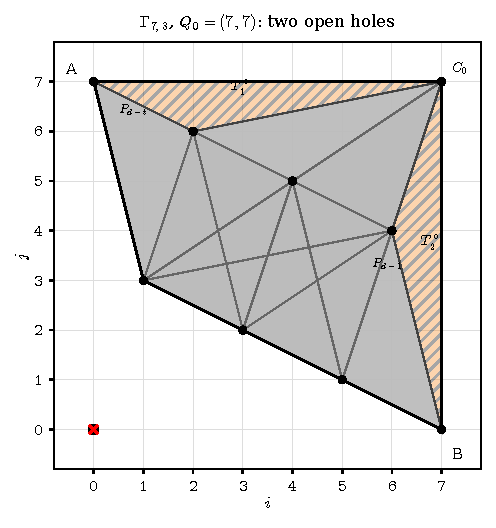
\includegraphics[width=.62\textwidth]{figures/fig03_two_holes.pdf}
\caption{The realized union in the exceptional box, $d=7$, $s=3$ ($t=5$), $Q_0=(7,7)$. Shaded: all admissible parallelograms. The segments are drawn in grey. The two white triangles $T_1=\conv(A,P_{d-t},C_0)$ and $T_2=\conv(B,P_{d-1},C_0)$ are not covered; their boundaries are.}\label{fig:two-holes}
\par\smallskip\noindent\figdesc{A square $[0,7]^2$ with the convex hull of the fibre outlined, many overlapping pale parallelograms covering most of it, and two white triangles near the top and right sides, both having the upper right corner $C_0=(7,7)$ as a vertex. The vertices $A$, $B$, $C_0$, $P_{d-t}$ and $P_{d-1}$ are labelled.}
\end{figure}

\subsection{The triangle interiors are not covered}

\begin{lemma}[Affine coordinates adapted to $T_1$]\label{lem:eta-xi}
Put $u=(c,-1)$ and $v=(d,0)$. For $p\in\Gamma$ write $p-A=\eta u+\xi v$. Then $\eta=d-p_y$ and $\xi=(p_x-\eta c)/d$ are integers. In the coordinates $(\eta,\xi)$, $A=(0,0)$, $P_{d-t}=(1,0)$, $C_0=(0,1)$ and $T_1$ is the triangle with vertices $(0,0),(1,0),(0,1)$.
\end{lemma}
\begin{proof}
The two equations $p_y-d=-\eta$ and $p_x=\eta c+\xi d$ give the stated formulas. Modulo $d$: $\eta c=(d-p_y)(d-t)\equiv tp_y\equiv tsp_x\equiv p_x$, so $d\mid p_x-\eta c$. The three vertex coordinates are immediate from $P_{d-t}-A=(c,-1)=u$ and $C_0-A=(d,0)=v$.
\end{proof}

\begin{proposition}[Exclusion of the open triangles]\label{prop:hole-exclusion}
For every $d\ge2$ and every unit $s$: $\partial T_1\subseteq U_0$ and $\interior T_1\cap U_0=\varnothing$. The same holds for $T_2$.
\end{proposition}
\begin{proof}
The inclusion $\partial T_1\subseteq U_0$ is \eqref{eq:dT1}. By Lemma~\ref{lem:T-transpose} it suffices to prove the exclusion for $T_1$. Work in the coordinates of Lemma~\ref{lem:eta-xi}. Then $\interior T_1=\{\eta>0,\xi>0,\eta+\xi<1\}$; every point of $F_{Q_0}$ has integer coordinates $(\eta,\xi)$ with $\eta=d-p_y\ge0$, so no point of $F_{Q_0}$ lies in $\interior T_1$ (``Step 0'').

\emph{Step 1: no admissible segment meets $\interior T_1$.} Let $[p,q]$ be an admissible segment with $q-p$ Graver, $p,q\in F_{Q_0}$, and suppose it contains a point of $\interior T_1$. Along the segment $\eta$ is affine and takes a value in $(0,1)$ at some point, while its endpoint values are integers $\ge0$. Hence one endpoint has $\eta=0$ and the other $\eta\ge1$. The points of $F_{Q_0}$ with $\eta=0$ (that is $p_y=d$) are $A=(0,0)_{\eta\xi}$ and $C_0=(0,1)_{\eta\xi}$ by Lemma~\ref{lem:exc-fibre}.

\emph{(a) The endpoint with $\eta=0$ is $A$.} Let $q=(\eta_q,\xi_q)$, $\eta_q\ge1$. The segment from $(0,0)$ to $q$ meets $\interior T_1$ only if some positive multiple $\theta q$ has $\theta\xi_q>0$ and $\theta(\eta_q+\xi_q)<1$; thus $\xi_q\ge1$. Then
\[
  q-A=\eta_qu+\xi_qv=(\eta_qc+\xi_qd,\ -\eta_q),
\]
and $u=(c,-1)$ satisfies $u\conf q-A$ (same signs, $c\le\eta_qc+\xi_qd$, $1\le\eta_q$), $u\in\Gamma$, $u\ne q-A$ because $\xi_q\ge1$. This contradicts the Graver property of $q-A$.

\emph{(b) The endpoint with $\eta=0$ is $C_0=(0,1)_{\eta\xi}$.} Let $q=(\eta_q,\xi_q)$ with $\eta_q\ge1$. A point $C_0+\theta(q-C_0)=(\theta\eta_q,\ 1+\theta(\xi_q-1))$, $0<\theta<1$, lies in $\interior T_1$ only if $\eta+\xi<1$, that is $\theta(\eta_q+\xi_q-1)<0$, so $\eta_q+\xi_q\le0$ as these are integers. Then $\xi_q\le-\eta_q$ and
\[
  q_x=\eta_qc+\xi_qd\le\eta_q(c-d)=-\eta_qt<0,
\]
which is impossible for a point of the box.

\emph{Step 2: no admissible parallelogram meets $\interior T_1$.} Let $P$ be an admissible parallelogram meeting $\interior T_1$. No vertex of $P$ is in $\interior T_1$ (Step 0), and no edge of $P$ meets $\interior T_1$ (Step 1, since edges are admissible segments). The set $\interior T_1$ is connected and disjoint from $\partial P$, so the nonempty set $\interior T_1\cap P$ is open and closed in $\interior T_1$, hence $\interior T_1\subseteq\interior P$. Then $A,C_0\in P$ and the segment $AC_0\subset P$. Since $P\subseteq[0,d]^2$ lies below the line $y=d$, $P\cap\{y=d\}$ is a face of $P$ containing the segment $AC_0$ of length $d$, so it is an edge of $P$ lying in $[0,d]\times\{d\}$ and containing $AC_0$, hence equal to $AC_0$. This edge is a Graver generator up to sign, namely $\pm(d,0)$. The other generator $h$ is independent and points downward ($h_y<0$) since $P\subseteq\{y\le d\}$. The other two corners are $A+h$ and $C_0+h$, which must lie in $[0,d]^2$, so $0\le h_x$ and $d+h_x\le d$, hence $h_x=0$ and $h=(0,-m)$ with $d\mid m$ (lattice condition) and $(0,-m)$ Graver, which forces $m=d$ by Lemma~\ref{lem:graver-size}. Then $A+h=(0,0)$, which is not in $F_{Q_0}$. Contradiction.

\emph{Conclusion.} $U_0$ is the union of admissible points, segments and parallelograms; none meets $\interior T_1$.
\end{proof}

\begin{remark}\label{rem:holes-lowerbound}
Proposition~\ref{prop:hole-exclusion} gives the lower bound $\beta_1(U_0)\ge 2$ in all classes where the two open triangles are bounded components of the complement (Section~\ref{sec:topology}). It does not, by itself, say that nothing else is missing from $H_0$; that is the content of the next section.
\end{remark}

%% -------------------------------------------------------------------
\section{Exact exceptional complement in nonspecial modular classes}\label{sec:nonspecial}

\begin{definition}[Nonspecial class]
The class $(d,s)$ is \emph{nonspecial} if $d\ge5$ and $2\le s\le d-2$ with $\gcd(s,d)=1$. Equivalently $a=d-s\ge2$, $c=d-t\ge2$, $s\ge2$, $t\ge2$. The classes $s\equiv\pm1$ are \emph{special}. For $d\in\{2,3,4,6\}$ every unit is special.
\end{definition}

\begin{theorem}[Nonspecial exceptional complement]\label{thm:exceptional}
If $d\ge5$, $2\le s\le d-2$ and $\gcd(s,d)=1$, then
\[
  \boxed{\,H_0\setminus U_0=\interior T_1\ \sqcup\ \interior T_2.\,}
\]
In particular $U_0=H_0\setminus(\interior T_1\cup\interior T_2)$, so $U_0$ is the closed polygon $H_0$ with two disjoint open triangles of area $d/2$ removed.
\end{theorem}

The proof has four ingredients: the lower-left chain of $H_0$ and its Graver steps (Lemma~\ref{lem:chain0}), a zonogon built from these steps and tiled by admissible parallelograms (Lemma~\ref{lem:zonogon}), one additional admissible cell $K$ (Lemma~\ref{lem:K}), and a covering argument (Lemma~\ref{lem:cover0}). The inclusion $\supseteq$ in the theorem is Proposition~\ref{prop:hole-exclusion}.

\subsection{The lower-left chain}

The boundary of $H_0$ consists of the segment $AC_0$ on $y=d$, the segment $C_0B$ on $x=d$ (both are in $H_0$ since $A,B,C_0\in F_{Q_0}$), and a convex arc from $A$ to $B$ on the lower-left, which we call the \emph{lower-left chain}.

\begin{lemma}[Lower-left chain]\label{lem:chain0}
Let $A=c_0,c_1,\dots,c_n=B$ be all lattice points of $\Gamma$ lying on the lower-left chain, in order along it, including collinear ones, and put $v_i=c_i-c_{i-1}=(a_i,-b_i)$. Then:
\begin{enumerate}
\item $a_i>0$ and $b_i>0$ for all $i$, and $b_1/a_1\ge b_2/a_2\ge\dots\ge b_n/a_n$;
\item every $v_i$ is a Graver vector;
\item $v_1=(1,s-d)=(1,-a)$ and $v_n=(d-t,-1)=(c,-1)$; in particular $n\ge2$ in a nonspecial class;
\item $\sum a_i=d$ and $\sum b_i=d$.
\end{enumerate}
\end{lemma}
\begin{proof}
(1) The chain is the graph of a convex function $f$ on $[0,d]$ with $f(0)=d$, $f(d)=0$ and $f\ge0$ on $[0,d]$ (the hull lies in the box). A convex function with $f(d)=0=\min f$ is nonincreasing, and it is strictly decreasing, since $f=0$ on an interval $[x_0,d]$, $x_0<d$, would put a lattice point $(i,0)$ with $0<i<d$ on the chain, but $(i,0)\in\Gamma$ forces $d\mid i$. Convexity gives nonincreasing $b_i/a_i$ (the slopes $-b_i/a_i$ are nondecreasing).

(2) Each pair $c_{i-1},c_i$ is a pair of consecutive boundary lattice points of $H_{Q_0}$ with $Q_0\ge(d,d)$; this is the boundary lemma (Lemma~\ref{lem:reflection}, Section~\ref{sec:reflection}, whose proof does not depend on the present section).

(3) Let $q=(q_x,q_y)\in F_{Q_0}$ with $q_x<d$, and write $B-q=(a',-b')$ with $a'=d-q_x\ge1$, $b'=q_y\ge0$. The last edge of the chain ends at $B$ and is the supporting line of $H_0$ at $B$ on the lower-left side, whose slope $b_n/a_n$ minimizes $b'/a'$ over all such $q$ (all of $H_0$ lies on or above this line). We claim that the minimum is attained at $q=(t,1)\in F_{Q_0}$, where $b'/a'=1/c$. Let $q\notin\{A\}$ (for $A$, $b'/a'=1\ge1/c$). Then $q=(d-a',b')$ with $1\le a'\le d-1$, $1\le b'\le d-1$, and the lattice condition $b'\equiv s(d-a')\equiv-sa'$ gives, after multiplying by $t$, $a'+tb'\equiv0\pmod d$. Write $tb'=md+r$ with $0\le r<d$. Since $t<d$ we have $m\le b'-1$. As $a'\ge1$ and $a'\equiv-r$, $r\neq0$ and $a'=d-r$. Then
\[
  b'c-a'=b'd-b't-d+r=(b'-m-1)d\ge0.
\]
Hence $a'\le b'c$, that is $b'/a'\ge1/c$, with equality exactly when $a'=b'c$. Points of equality lie on the line through $B$ with direction $(c,-1)$; the lattice point of this line nearest to $B$ is $(t,1)$, since $a'=b'c\ge c$ with equality only for $b'=1$. So $(t,1)$ is the lattice point preceding $B$ on the chain and $v_n=B-(t,1)=(c,-1)$. Transposition (Proposition~\ref{prop:elem}(5)) turns this into the statement for the first step: in $\Gamma_{d,t}$ the last step into $B$ is $(d-s,-1)$, and transposing and reversing gives the first step $v_1=(1,-(d-s))=(1,s-d)$ in $\Gamma_{d,s}$. Finally $(1,-a)=(c,-1)$ would force $a=c=1$, that is $s=t=d-1$, a special class; hence $v_1\ne v_n$ and $n\ge2$ in a nonspecial class.

(4) $c_0=A$ and $c_n=B$.
\end{proof}

\subsection{The zonogon}

Let $Z=A+\sum_{i=1}^n[0,v_i]$ be the zonogon generated by the chain steps. Its lower-left boundary is the chain (steps in the order $v_1,\dots,v_n$, steep to shallow) and its upper-right boundary is the chain with steps in the reverse order $v_n,\dots,v_1$.

\begin{lemma}[Zonogon cover]\label{lem:zonogon}
Let $d\ge5$ be nonspecial. There is a finite family of admissible parallelograms with vertex sets in $\{A+\sum_{i\in S}v_i:S\subseteq\{1,\dots,n\}\}$ whose union is $Z$. In particular $Z\subseteq U_0$.
\end{lemma}
\begin{proof}
\emph{All subset sums are admissible corners.} For $S\subseteq\{1,\dots,n\}$ the point $z_S=A+\sum_{i\in S}v_i$ lies in $\Gamma$ (a sum of lattice vectors), and its coordinates are $x=\sum_{i\in S}a_i\in[0,d]$, $y=d-\sum_{i\in S}b_i\in[0,d]$, by Lemma~\ref{lem:chain0}(4). If $z_S=0$ then $x=0$ forces $S=\varnothing$, giving $z_S=A\ne0$. So $z_S\in F_{Q_0}$ for every $S$.

\emph{Sweeping construction.} Put $Z_k=A+\sum_{i\le k}[0,v_i]$. We show by induction on $k$ that $Z_k$ is covered by admissible parallelograms with corners among the subset sums. For $k=1$ the set $Z_1$ is the Graver segment $[A,A+v_1]$, which is admissible. Let $k\ge2$ and assume the claim for $Z_{k-1}$. Put $\psi(z)=\cross(v_k,z)=a_kz_y+b_kz_x$. For $i<k$ the slope ordering gives
\[
  \psi(v_i)=b_ka_i-a_kb_i\le0,\quad\text{with equality exactly when }v_i\parallel v_k.
\]
Hence over $Z_{k-1}$ the functional $\psi$ has its maximum at $A$ and its minimum at $A+\sum_{i<k}v_i$, and the boundary of $Z_{k-1}$ splits at these two points into the lower-left chain, with edges $v_1,\dots,v_{k-1}$ in this order, and the upper-right chain, with edges $v_{k-1},\dots,v_1$ in this order from $A$. An edge of direction $v_i$ on the upper-right chain has outward normal $n=(b_i,a_i)$ and $n\cdot v_k=-\psi(v_i)\ge0$; on the lower-left chain the outward normal $(-b_i,-a_i)$ has $n\cdot v_k=\psi(v_i)\le0$.

For a convex polygon $P$ and a vector $v$ one has $P+[0,v]=P\cup\bigcup_e\,(e+[0,v])$, the union over the edges $e$ whose outward normal $n$ satisfies $n\cdot v>0$. (If $z\in P$, $0<\theta\le1$ and $z+\theta v\notin P$, the ray from $z$ in direction $v$ leaves $P$ at a point $z'$ of such an edge and $z+\theta v=z'+\lambda v$ with $0<\lambda\le1$; the converse inclusion is clear.) Here the relevant edges are the edges of the upper-right chain not parallel to $v_k$. Each such edge, $e=[w,w+v_i]$ with $w$ a subset sum, sweeps the parallelogram $e+[0,v_k]=P(w;v_i,v_k)$, whose four corners are subset sums, whose generators $v_i,v_k$ are Graver (Lemma~\ref{lem:chain0}(2)) and independent. Edges parallel to $v_k$ sweep nothing. So $Z_k=Z_{k-1}\cup\bigcup P(w;v_i,v_k)$ is covered by admissible parallelograms. Repeated parallel steps cause no difficulty: they produce collinear boundary edges and no new tiles.

For $k=n$ we get $Z_n=Z$.
\end{proof}

\begin{figure}[ht]
\centering
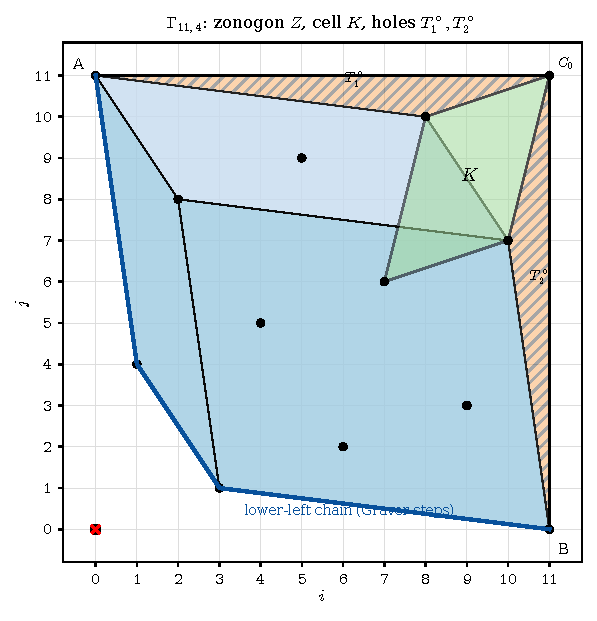
\includegraphics[width=.7\textwidth]{figures/fig04_zonogon.pdf}
\caption{$d=11$, $s=4$ ($t=3$): the zonogon $Z$ (blue tiles, alternating shades) generated by the Graver steps of the lower-left chain (thick blue), the extra cell $K$ (orange) and the two open triangles $T_1^\circ,T_2^\circ$ (white). Together they cover $H_0$.}\label{fig:zonogon}
\par\smallskip\noindent\figdesc{A square $[0,11]^2$ with the lower-left chain from $A=(0,11)$ to $B=(11,0)$ drawn thick; the zonogon it generates is tiled by parallelograms of two alternating blue shades; one orange parallelogram $K$ sits near the upper right corner between the zonogon's upper chain and $C_0$; two white triangles with vertex $C_0$ complete the hull.}
\end{figure}

\subsection{\texorpdfstring{The additional cell $K$}{The additional cell K}}

\begin{lemma}[The cell $K$]\label{lem:K}
For a nonspecial class put $w_K=(c-1,\ a-1)$ and
\[
  K=P\bigl(w_K;\ (1,s),\ (t,1)\bigr).
\]
Its corners are $w_K$, $L=P_{d-t}=(c,d-1)$, $R=P_{d-1}=(d-1,a)$ and $C_0$. The cell $K$ is admissible, so $K\subseteq U_0$.
\end{lemma}
\begin{proof}
$w_K+(1,s)=(c,a-1+s)=(c,d-1)=L$, $w_K+(t,1)=(c-1+t,a)=(d-1,a)=R$, and $w_K+(1,s)+(t,1)=(c+t,a+s)=(d,d)=C_0$. In a nonspecial class $c\ge2$ and $a\ge2$, so $w_K$ has positive coordinates; it lies in $\Gamma$ because $w_K=L-(1,s)$, and in the box. The four corners are in $F_{Q_0}$. The generators $(1,s)$ and $(t,1)$ are Graver (Lemma~\ref{lem:std-graver}) with $\cross((1,s),(t,1))=1-st$, which is nonzero since $s,t\ge2$ give $st\ge4$.
\end{proof}

\subsection{Covering}

\begin{lemma}[Covering of $H_0$]\label{lem:cover0}
In a nonspecial class, $H_0\subseteq Z\cup T_1\cup T_2\cup K$.
\end{lemma}
\begin{proof}
For $0\le x\le d$ the vertical slice of $H_0$ is $[f(x),g(x)]$, where $f$ is the lower-left chain, $g(x)=d$ for $0\le x<d$ (the side $AC_0$) and the slice at $x=d$ is $[0,d]$ (the side $C_0B$). The vertical slice of $Z$ is $[f(x),h(x)]$, where $h$ is the concave function whose graph is the upper-right chain of $Z$. This chain begins with the edge from $A$ to $A+v_n=L=(c,d-1)$ and ends with the edge from $R=B-v_1=(d-1,a)$ to $B$ (Lemma~
ef{lem:chain0}(3)). Let $z\in H_0\setminus Z$; then $h(z_x)<z_y\le g(z_x)$. Write $E_1=(c,d)$ and $E_2=(d,a)$; these are points of the sides $AC_0$ and $C_0B$.

\emph{Region I: $z_x\le c$.} On $[0,c]$ the function $h$ is the segment $AL$, so $z$ lies on or above $AL$ and on or below $y=d$, that is in the triangle $\conv(A,L,E_1)\subseteq T_1$.

\emph{Region II: $z_y\le a$.} The upper-right chain of $Z$ is monotone (the abscissa increases and the ordinate decreases along it), so horizontal slices of $Z$ are intervals, and on the heights $0\le y\le a$ its right end is the segment $RB$. A point $z\in H_0\setminus Z$ with $z_y\le a$ therefore lies to the right of the segment $RB$ and to the left of $x=d$: in the triangle $\conv(B,R,E_2)\subseteq T_2$.

\emph{Region III: $z_x>c$ and $z_y>a$.} Then $z\in[c,d]\times[a,d]$. We claim that $z$ lies on or above the line $LR$. If $c<z_x\le d-1$, $z$ lies above the concave chain of $Z$ from $L$ to $R$, which lies on or above the chord $LR$. If $z_x>d-1$ then $z_y>a$, and the line $LR$ has ordinate below $a$ there. Now the part of the rectangle $[c,d]\times[a,d]$ on or above the line $LR$ is the convex pentagon with vertices $L,E_1,C_0,E_2,R$, which is the union of the three triangles $\conv(C_0,L,E_1)$, $\conv(C_0,L,R)$, $\conv(C_0,R,E_2)$. The first is contained in $T_1$ (its vertices lie in $T_1$), the third in $T_2$, and the second is $\Delta=\conv(L,R,C_0)\subseteq K$ since three of the corners of the parallelogram $K$ are $L,R,C_0$ (Lemma~\ref{lem:K}).

The three regions exhaust $H_0\setminus Z$.
\end{proof}

\begin{proof}[Proof of Theorem~\ref{thm:exceptional}]
By Lemmas~\ref{lem:zonogon} and \ref{lem:K}, $Z\cup K\subseteq U_0$. By \eqref{eq:dT1}, $\partial T_i\subseteq U_0$. By Lemma~\ref{lem:cover0}, every point of $H_0\setminus U_0$ lies in $T_1\cup T_2$ and not in $\partial T_1\cup\partial T_2$; hence $H_0\setminus U_0\subseteq\interior T_1\cup\interior T_2$. Conversely $T_i\subseteq H_0$ because the vertices of $T_i$ are in $F_{Q_0}$, and $\interior T_i\cap U_0=\varnothing$ by Proposition~\ref{prop:hole-exclusion}. The two open triangles are disjoint by Lemma~\ref{lem:T-disjoint}.
\end{proof}

\begin{remark}[Both inclusions]
The theorem is an equality of sets: the inclusion $H_0\setminus U_0\subseteq\interior T_1\sqcup\interior T_2$ is the covering argument (Lemmas~\ref{lem:zonogon}--\ref{lem:cover0}), and the reverse inclusion is the exclusion argument (Proposition~\ref{prop:hole-exclusion}), which includes the treatment of the deleted origin.
\end{remark}

\begin{remark}[Modular sail]
The lower-left chain of $H_0$ is the part between $A$ and $B$ of the boundary of $\conv\bigl(\Gamma\cap\R_{\ge0}^2\setminus\{0\}\bigr)$, the Klein sail of the lattice in the quadrant (Proposition~\ref{prop:persist} below shows that every nonzero lattice point of the quadrant lies on the upper-right side of each supporting line of the chain). The chain steps in Lemma~\ref{lem:chain0} are the consecutive vectors of this sail. For the lattice $\Gamma_{d,s}$ the sail is governed by the continued fraction of $s/d$; we do not use this.
\end{remark}

\begin{remark}[The cells overlap]
The union $Z\cup K\cup T_1\cup T_2$ is a cover, not a tiling. For $(d,s)=(5,2)$ the zonogon has area $10$, $K$ has area $5$ and $T_1,T_2$ have area $2.5$ each; the hull has area $17.5$, so $K$ overlaps $Z$ in area $2.5$ (the part of $K$ below the chord $LR$ of Lemma~\ref{lem:cover0}).
\end{remark}

%% -------------------------------------------------------------------
\section{Special modular classes and exceptional configurations}\label{sec:special-classes}

The classes $s\equiv-1$ and $s\equiv+1\pmod d$ are treated separately: they have different fibres, different Graver bases and, for $s\equiv-1$, different topology. Both rely on the complete lists of Graver vectors proved in Lemma~\ref{lem:special-graver} (Section~\ref{sec:special-stab}, whose proof does not depend on the present section).

\subsection{\texorpdfstring{The class $s\equiv-1$: the fan graph}{The class s = -1: the fan graph}}

Let $s=d-1$, so $t=d-1$, $\Gamma=\{(i,j):i+j\equiv0\ (\mathrm{mod}\ d)\}$.

\begin{proposition}[The fan graph]\label{prop:special-fan}
For $s=d-1$ and $d\ge2$, $F_{Q_0}=\{E_0,\dots,E_d\}\cup\{C_0\}$ with $E_i=(i,d-i)$ (so $E_0=A$, $E_d=B$). The set $U_0$ is the union of the $d$ segments $[E_{i-1},E_i]$ and the $d+1$ spokes $[E_i,C_0]$. It is a connected planar graph with $d+2$ vertices and $2d+1$ edges, containing no two-dimensional cell, with
\[
  \beta_1(U_0)=d,\qquad\beta_2(U_0)=0.
\]
The complement $H_0\setminus U_0$ is the disjoint union of the $d$ open triangles $\interior\conv(E_{i-1},E_i,C_0)$, each of area $d/2$; $T_1$ and $T_2$ are two of them.
\end{proposition}
\begin{proof}
A point $(i,j)\in\Gamma\cap[0,d]^2\setminus\{0\}$ has $i+j\in\{d,2d\}$, giving the antidiagonal points $E_0,\dots,E_d$ and the single point $C_0=(d,d)$. By Lemma~\ref{lem:special-graver} the Graver vectors are $\pm(1,-1)$ and $\pm(k,d-k)$, $0\le k\le d$. Then $E_i-E_{i-1}=(1,-1)$ is Graver, whereas $E_j-E_i=(j-i)(1,-1)$ for $j-i\ge2$ is not (it has $(1,-1)$ conformally below it); and $C_0-E_i=(d-i,i)=(k,d-k)$ with $k=d-i$ is Graver. So the admissible segments are the stated ones (and unions of them).

No admissible parallelogram exists: the four corners of a nondegenerate parallelogram have no three collinear, but any four points of $F_{Q_0}$ contain at least three of the collinear points $E_i$.

Thus $U_0$ is the union of the antidiagonal segment $[A,B]$ (subdivided at the $E_i$) and the spokes. A spoke meets the line $x+y=d$ only at its endpoint $E_i$, because $C_0$ is off that line; spokes meet one another only at $C_0$. So $U_0$ is an embedded graph with $V=d+2$ vertices and $E=d+(d+1)=2d+1$ edges. It is connected, hence $\beta_1=E-V+1=d$. A graph has no $H_2$.

The hull $H_0=\conv(A,B,C_0)$ has area $d^2/2$. The $d$ triangles $\conv(E_{i-1},E_i,C_0)$ form a fan from $C_0$ over the subdivided side $[A,B]$, so they have disjoint interiors and their union is $H_0$; each has area $\tfrac12|\cross(E_i-E_{i-1},\,C_0-E_{i-1})|=\tfrac12|\cross((1,-1),(d-i+1,i-1))|=d/2$. Each is bounded by edges of the graph, so the interiors are the components of $H_0\setminus U_0$. For $s=t=d-1$ we have $P_{d-t}=P_1=E_1$ and $P_{d-1}=E_{d-1}$, so $T_1=\conv(A,E_1,C_0)$ and $T_2=\conv(B,E_{d-1},C_0)$ are the first and last of these triangles.
\end{proof}

\subsection{\texorpdfstring{The class $s\equiv+1$ with $d\ge3$: the exact complement}{The class s = +1 with d >= 3: the exact complement}}

\begin{remark}[Source status]\label{rem:s1-source}
The identity $\beta_1(U_0)=2$ for $s\equiv+1$, $d\ge3$ is recorded in the GEO-I releases (v005, G5-C2). The exact description of the \emph{complement} $H_0\setminus U_0$ given in Proposition~\ref{prop:special-plus} below, and its proof from the explicit cell list, were derived in the working draft preceding this manuscript (the ``v2 mathematical core'') and are not attributed to v005 as a theorem stated there. In the v005 notation the roles of $A$ and $B$ are interchanged.
\end{remark}

Let $s=1$, $t=1$, $\Gamma=\{(i,j):j\equiv i\ (\mathrm{mod}\ d)\}$, $d\ge3$. Put $D_i=(i,i)$ for $1\le i\le d$, so $D_d=C_0$. By Lemma~\ref{lem:exc-fibre}, $F_{Q_0}=\{A,B,D_1,\dots,D_d\}$, and $P_i=D_i$.

\begin{proposition}[The class $s=1$]\label{prop:special-plus}
Let $s=1$, $d\ge3$ and
\[
  W=P\bigl(A;\ (1,1-d),\ (d-1,-1)\bigr)=\conv(A,D_1,B,D_{d-1}).
\]
Then $W$ is an admissible parallelogram and
\[
  U_0=W\ \cup\ [A,C_0]\ \cup\ [B,C_0]\ \cup\ [D_{d-1},C_0],\qquad
  H_0\setminus U_0=\interior T_1\ \sqcup\ \interior T_2,
\]
where $T_1=\conv(A,D_{d-1},C_0)$ and $T_2=\conv(B,D_{d-1},C_0)$ share the edge $[D_{d-1},C_0]$. Consequently $\beta_1(U_0)=2$ and $\beta_2(U_0)=0$.
\end{proposition}
\begin{proof}
\emph{$W$ is admissible.} $(1,1-d)$ and $(d-1,-1)$ are Graver by Lemma~\ref{lem:special-graver} (they are the vectors $\pm(k,-(d-k))$ with $k=1$ and $k=d-1$) and independent: $\cross=-1+(d-1)^2=d(d-2)\ne0$ for $d\ge3$. The corners are $A$, $A+(1,1-d)=D_1$, $A+(d-1,-1)=D_{d-1}$, $A+(d,-d)=B$, all in $F_{Q_0}$.

\emph{Parallelograms.} A nondegenerate parallelogram has no three collinear corners, but the $D_i$ are collinear; so its corners include at most two $D_i$, hence both $A$ and $B$ and two points $D_i,D_j$. If $D_i,D_j$ were adjacent corners then so would be $A,B$, and the sides $AB$ and $D_iD_j$ would be parallel, but $AB$ has direction $(1,-1)$ and $D_iD_j$ has direction $(1,1)$. So $D_i,D_j$ are opposite corners, and so are $A,B$; the diagonals bisect each other, so $D_i+D_j=A+B=(d,d)$, i.e. $i+j=d$. Each such parallelogram $\conv(A,D_i,B,D_{d-i})$ is contained in $W=\conv(A,D_1,B,D_{d-1})$, because $D_i,D_{d-i}\in[D_1,D_{d-1}]$. So the union of the admissible parallelograms is exactly $W$.

\emph{Segments.} By Lemma~\ref{lem:special-graver}: $D_{i+1}-D_i=(1,1)$ is Graver, but $D_j-D_i$ for $j-i\ge2$ is not. The segments $[D_i,D_{i+1}]$ for $i\le d-2$ lie in $W$ (they are in $[D_1,D_{d-1}]$), and $[D_{d-1},C_0]$ does not lie in $W$. For $i\le d-1$, $D_i-A=(i,i-d)$ and $D_i-B=(i-d,i)$ are Graver (the vectors $\pm(k,-(d-k))$), and the segments $[A,D_i]$, $[B,D_i]$ lie in $W$ by convexity ($A,B,D_i\in W$). $B-A=(d,-d)$ is not Graver, since $(1,1-d)\in\Gamma$ satisfies $(1,1-d)\conf(d,-d)$ and differs from it for $d\ge3$. Finally $C_0-A=(d,0)$ and $C_0-B=(0,d)$ are Graver, giving $[A,C_0]$ and $[B,C_0]$; $C_0-D_i$ for $i<d-1$ is $(d-i)(1,1)$ with $d-i\ge2$, not Graver. The admissible segments outside $W$ are therefore exactly $[A,C_0]$, $[B,C_0]$, $[D_{d-1},C_0]$. This gives the stated formula for $U_0$.

\emph{The complement.} The hull is the quadrilateral $H_0=\conv(A,D_1,B,C_0)$. The diagonal from $D_1$ to $C_0$ passes through $D_{d-1}$ and cuts $H_0$ into the triangles $\conv(A,D_1,C_0)$ and $\conv(B,D_1,C_0)$. Cutting the first along $[A,D_{d-1}]$ gives $\conv(A,D_1,D_{d-1})\cup T_1$ and cutting the second along $[B,D_{d-1}]$ gives $\conv(B,D_1,D_{d-1})\cup T_2$. The two triangles $\conv(A,D_1,D_{d-1})$ and $\conv(B,D_1,D_{d-1})$ make up $W$. Hence $H_0=W\cup T_1\cup T_2$ with $W,T_1,T_2$ having pairwise disjoint interiors. The boundaries of $T_1,T_2$ lie in $U_0$ by \eqref{eq:dT1}, and their interiors are disjoint from $U_0$ by Proposition~\ref{prop:hole-exclusion} (here $T_1=\conv(A,P_{d-1},C_0)$ since $t=1$). So $H_0\setminus U_0=\interior T_1\sqcup\interior T_2$.

The Betti numbers follow from the topology of Section~\ref{sec:topology} (Theorem~\ref{thm:betti}).
\end{proof}

\begin{figure}[ht]
\centering
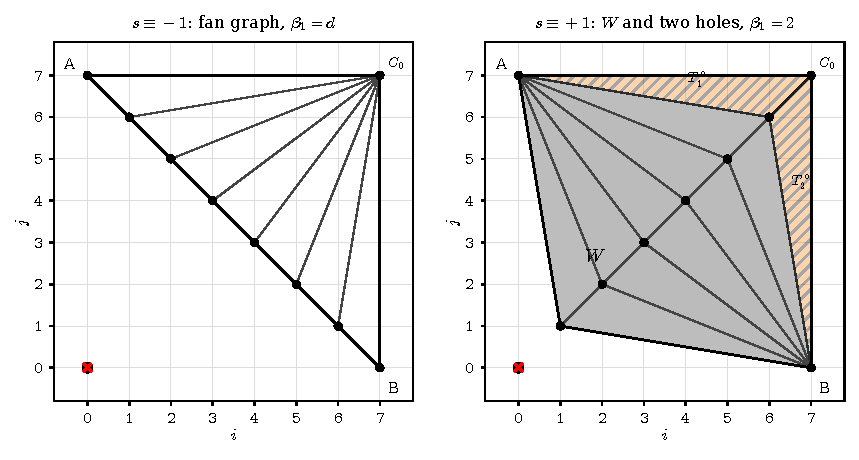
\includegraphics[width=\textwidth]{figures/fig05_special.pdf}
\caption{The two special exceptional configurations for $d=7$. Left: $s\equiv-1$, the fan graph with $d$ bounded triangles ($\beta_1=7$). Right: $s\equiv+1$, the parallelogram $W$, the segments $[A,C_0]$, $[B,C_0]$, $[D_{d-1},C_0]$, and the two open triangles $T_1,T_2$ ($\beta_1=2$).}\label{fig:special}
\par\smallskip\noindent\figdesc{Two panels, each a square $[0,7]^2$. Left: the antidiagonal from $A=(0,7)$ to $B=(7,0)$ with eight points and seven spokes from the upper-right corner $C_0$, no shaded regions. Right: a shaded parallelogram $W$ with vertices $A$, $(1,1)$, $B$, $(6,6)$, plus segments from $C_0$ to $A$, to $B$ and to $(6,6)$, with two white triangles beside $C_0$.}
\end{figure}

\subsection{\texorpdfstring{The overlap at $d=2$}{The overlap at d = 2}}

For $d=2$ the only unit is $1\equiv-1$. Then $F_{Q_0}=\{A=(0,2),\ P_1=(1,1),\ B=(2,0),\ C_0=(2,2)\}$, and the fan description of Proposition~\ref{prop:special-fan} applies: the edges are $[A,P_1]$, $[P_1,B]$ and the spokes $[A,C_0]$, $[P_1,C_0]$, $[B,C_0]$, a graph with four vertices and five edges, so $\beta_1=d=2$. The complement is $\interior T_1\sqcup\interior T_2$ with $T_1=\conv(A,P_1,C_0)$ and $T_2=\conv(B,P_1,C_0)$ of area $1$ each. Thus at $d=2$ the two special descriptions coincide in outcome: $\beta_1=2=d$, and the $s\equiv+1$ construction (which needs $d\ge3$ because $W$ degenerates to a segment) is not used.

\begin{table}[ht]
\centering\small
\begin{tabular}{@{}lll@{}}
\toprule
Class & $U_0$ & $\beta_1(U_0)$\\
\midrule
$d\ge5$, $2\le s\le d-2$ & $H_0$ minus two open triangles & $2$\\
$s\equiv+1$, $d\ge3$ & $W\cup$ three segments; $H_0$ minus two open triangles & $2$\\
$s\equiv-1$, $d\ge3$ & fan graph, no $2$-cells & $d$\\
$d=2$ ($s=1$) & fan graph with $4$ vertices & $2$\\
\bottomrule
\end{tabular}
\caption{Exceptional topology $U_{d,s,(d,d)}$ by modular class (rational coefficients; justified in Section~\ref{sec:topology}).}\label{tab:betti}
\end{table}

%% -------------------------------------------------------------------
\section{Topology, homology and geometric interpretation}\label{sec:topology}

\subsection{Planar topology}

We use Alexander duality in the following form.

\begin{theorem}[Alexander duality; Hatcher, \emph{Algebraic Topology}, Theorem~3.44, \S3.3]\label{thm:alexander}
Let $X$ be a nonempty compact, locally contractible proper subspace of $S^2$. Then $\tilde H_i(S^2\setminus X;\Z)\cong\tilde H^{\,1-i}(X;\Z)$ for all $i$.
\end{theorem}

A compact polyhedron in the plane is locally contractible. We use rational coefficients, where cohomology and homology ranks agree.

\begin{corollary}[Betti numbers of a planar polyhedron]\label{cor:planar-betti}
Let $X\subset\R^2$ be a nonempty compact polyhedron. Then $\beta_1(X)$ equals the number of bounded connected components of $\R^2\setminus X$, and $\beta_2(X)=0$.
\end{corollary}
\begin{proof}
Regard $\R^2\subset S^2=\R^2\cup\{\infty\}$. The set $S^2\setminus X$ is nonempty (it contains $\infty$), and $X$ is a proper compact locally contractible subspace of $S^2$. Theorem~\ref{thm:alexander} with $i=0$ gives $\tilde H_0(S^2\setminus X;\Q)\cong\tilde H^1(X;\Q)$, so $S^2\setminus X$ has exactly $1+\beta_1(X)$ components. One of them contains $\infty$ and the others are the bounded components of $\R^2\setminus X$.

For $\beta_2$, triangulate $X$ and let $z=\sum_\sigma c_\sigma\sigma$ be a $2$-cycle, the $\sigma$ being $2$-simplices of the triangulation oriented as in the plane. Suppose $z\ne0$. Choose a linear functional $\Phi$ on $\R^2$ that is not constant on any edge, and let $v$ be a vertex maximizing $\Phi$ among the vertices of simplices with $c_\sigma\ne0$. At $v$ the simplices of the support of $z$ occupy angular wedges with disjoint interiors, all in the half-plane $\{\Phi\le\Phi(v)\}$ (all their other vertices have smaller $\Phi$). Let $e$ be the edge along the most clockwise bounding ray of the union of these wedges. The simplex $\sigma$ of the support containing $e$ lies counterclockwise from $e$, and no other simplex of the support contains $e$ (it would lie clockwise from $e$). So the coefficient of $e$ in $\partial z$ is $\pm c_\sigma\ne0$, contradicting $\partial z=0$. Hence $H_2(X;\Q)=0$.
\end{proof}

\subsection{Betti numbers of the exceptional union}

\begin{theorem}[Exceptional topology]\label{thm:betti}
$U_0=U_{d,s,(d,d)}$ is connected with $\beta_2(U_0)=0$ and
\[
  \beta_1(U_0)=\begin{cases}
  d & s\equiv-1\pmod d,\\
  2 & \text{otherwise }(d\ge2).
  \end{cases}
\]
(For $d=2$ the two cases coincide, $\beta_1=2=d$.)
\end{theorem}
\begin{proof}
\emph{$s\equiv-1$:} Proposition~\ref{prop:special-fan}.

\emph{Otherwise:} in a nonspecial class and for $s=1$, $d\ge3$, we have $H_0\setminus U_0=\interior T_1\sqcup\interior T_2$ (Theorem~\ref{thm:exceptional}, Proposition~\ref{prop:special-plus}). Then
\[
  \R^2\setminus U_0=(\R^2\setminus H_0)\ \sqcup\ \interior T_1\ \sqcup\ \interior T_2.
\]
Each piece is open and connected: $\R^2\setminus H_0$ is the complement of a compact convex set in the plane, and the triangle interiors are convex. The boundary of each piece is contained in $U_0$: $\partial H_0$ consists of the lower-left chain (in $Z$, resp. in $W$), $[A,C_0]$ and $[B,C_0]$ (edges of $T_1$, $T_2$), all in $U_0$; and $\partial T_i\subseteq U_0$ by \eqref{eq:dT1}. A connected open subset of $\R^2\setminus U_0$ whose boundary lies in $U_0$ is a full component. Therefore $\R^2\setminus U_0$ has exactly three components, of which two are bounded, and Corollary~\ref{cor:planar-betti} gives $\beta_1=2$, $\beta_2=0$. Connectedness: $U_0=Z\cup K\cup\partial T_1\cup\partial T_2$ in a nonspecial class, and these four connected sets meet consecutively ($A\in Z\cap\partial T_1$, $L\in\partial T_1\cap K$, $R\in K\cap\partial T_2$); for $s=1$ it is $W\cup[A,C_0]\cup[B,C_0]\cup[D_{d-1},C_0]$, connected through $A,B,D_{d-1}$. For $d=2$ use Proposition~\ref{prop:special-fan}.
\end{proof}

\subsection{Interpretation: fan versus two holes}

The two exceptional configurations are of different kinds.

\begin{itemize}
\item In the \emph{fan} ($s\equiv-1$) the realized union is one-dimensional. The Graver vectors of $\Gamma_{d,d-1}$ include every $(k,d-k)$, so every fibre point is joined to $C_0$, but the point set has only one point off a line; there is no way to span a nondegenerate parallelogram. The first Betti number counts the $d$ triangular faces of the graph and grows with $d$.
\item In the \emph{two-hole} classes the union is a polygon with two triangular punctures, of fixed first Betti number $2$ independent of $d$ and $s$. The two triangles are the only part of the hull not covered, they have a common vertex $C_0$, and each has area $d/2$, one half of a fundamental parallelogram of $\Gamma$.
\end{itemize}

\begin{remark}[What the topology is a topology of]\label{rem:topology-scope}
The Betti numbers in Theorem~\ref{thm:betti} are Betti numbers of the compact set $U_0$ defined in Section~\ref{sec:cells}. They are not asserted to be forced by occurrence arithmetic: the arithmetic supplies the points and their exact Graver relations, and the cell attachment rule (Remark~\ref{rem:modelling}) is a modelling choice. The abstract complex $K_{\mathrm{abs}}$ of Definition~\ref{def:kabs} has the same underlying set as $U_0$ only after the identification $\pi$; its Betti numbers may differ, for instance if two distinct cells share a boundary and overlap. Statements about the topology of an occurrence fibre are statements about $U_Q$.
\end{remark}

%% -------------------------------------------------------------------
\section{Enlargement and filling of the exceptional holes}\label{sec:fill}

We now show what happens to the two exceptional triangles when the box is enlarged by even one step.

\begin{proposition}[Hole filling]\label{prop:fill}
Let $d\ge3$ and let $s$ be any unit modulo $d$. For every box $Q\ge(d,d)$ with $Q\ne(d,d)$, both closed triangles $T_1,T_2$ lie in $U_Q$.
\end{proposition}
\begin{proof}
By transposition (Proposition~\ref{prop:elem}(5) and Lemma~\ref{lem:T-transpose}) it suffices to treat $Q_2\ge d+1$: if $Q_2=d$ then $Q_1\ge d+1$, and the transposed instance has $Q'_2=Q_1\ge d+1$ and $T_1,T_2$ exchanged.

Let $Q_2\ge d+1$ and put
\[
  R_1=P\bigl(A;\ (c,-1),\ (t,1)\bigr),\qquad R_2=P\bigl((t,1);\ (0,d),\ (c,-1)\bigr).
\]
The generators are Graver by Lemma~\ref{lem:std-graver}, and independent: $\cross((c,-1),(t,1))=c+t=d$ and $\cross((0,d),(c,-1))=-dc\ne0$. The corners of $R_1$ are $A$, $A+(c,-1)=P_{d-t}$, $A+(t,1)=(t,d+1)$ and $A+(d,0)=C_0$; the corners of $R_2$ are $(t,1)$, $(t,d+1)$, $(t,1)+(c,-1)=B$ and $(t,1)+(0,d)+(c,-1)=C_0$. All lie in $\Gamma$, are nonzero, and lie in $[0,d]\times[0,d+1]\subseteq[0,Q_1]\times[0,Q_2]$.

Three corners of $R_1$ are the vertices $A,P_{d-t},C_0$ of $T_1$, so $T_1\subseteq R_1\subseteq U_Q$. Two corners of $R_2$ are $B,C_0$. To see $P_{d-1}=(d-1,a)\in R_2$: write $(d-1,a)=(t,1)+\alpha(0,d)+\beta(c,-1)$. The first coordinate gives $\beta=(d-1-t)/c=(c-1)/c\in[0,1)$ and the second $\alpha=\bigl(a-1+\beta\bigr)/d$. Since $a\ge1$ and $a-1+\beta<a\le d-1$, $\alpha\in[0,1]$. So all vertices of $T_2$ lie in the convex set $R_2$, whence $T_2\subseteq R_2\subseteq U_Q$.
\end{proof}

\begin{figure}[ht]
\centering
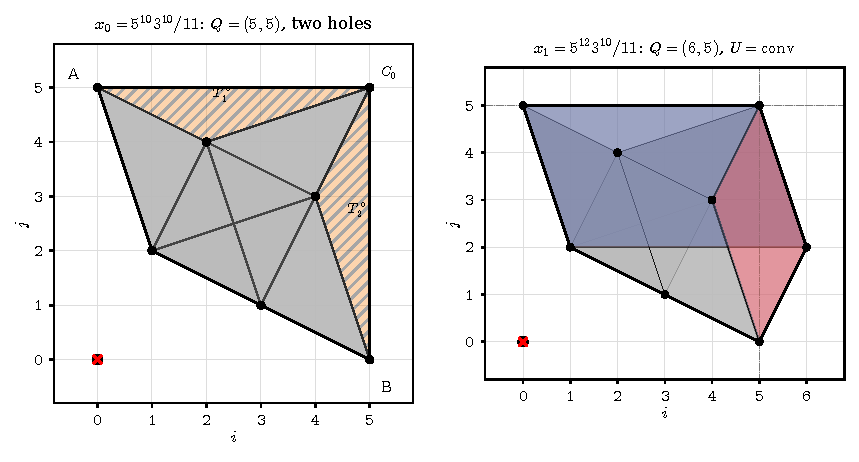
\includegraphics[width=\textwidth]{figures/fig12_example.pdf}
\caption{Hole filling in the running example $(d,s)=(5,2)$ ($t=3$). Left: the exceptional box $Q_0=(5,5)$ with its two white triangles. Right: the box $(6,5)$; the filling cells $R_1,R_2$ are among the cells drawn, together with the cap cells of Part~III. This is the same pair of occurrence fibres as in Section~\ref{sec:example}.}\label{fig:fill-preview}
\par\smallskip\noindent\figdesc{Two side-by-side panels. Left, box $5\times5$: pale parallelograms cover the hull of seven points except two white triangles at the upper right. Right, box $6\times5$: coloured parallelograms cover the entire hull of eight points.}
\end{figure}

\subsection{Old-hull coverage and the dependency chain}

The filling proposition alone does not show that the old hull is covered: one must know what else is missing from $H_0$. In the GEO-I record this was organised as follows.

\begin{itemize}
\item \textbf{G8-T1} is Proposition~\ref{prop:fill}.
\item \textbf{G8-R1} (v008) is the reduction ``$H_0\subseteq U_Q$ for $Q\ge(d,d)$, $Q\ne(d,d)$'' \emph{conditional} on the premise that the complement of $U_0$ in $H_0$ is contained in $T_1\cup T_2$ (called G8-T2 there).
\item The premise is the covering half of the exact complement theorem (v010: G10-Z, G10-T1), which is Theorem~\ref{thm:exceptional} above, together with Proposition~\ref{prop:special-plus} for $s=1$. Combining it with G8-T1 makes G8-R1 unconditional (G10-R1).
\end{itemize}

We give the argument in full.

\begin{corollary}[Old-hull coverage]\label{cor:old}
Let $Q\ge(d,d)$, $Q\ne(d,d)$. If the class is nonspecial, or $s=1$ with $d\ge3$, then $H_0\subseteq U_Q$.
\end{corollary}
\begin{proof}
Every cell admissible for $Q_0$ is admissible for $Q$ (Proposition~\ref{prop:elem}(4)), so $U_0\subseteq U_Q$. By Theorem~\ref{thm:exceptional} (nonspecial) or Proposition~\ref{prop:special-plus} ($s=1$), $H_0\setminus U_0=\interior T_1\sqcup\interior T_2\subseteq T_1\cup T_2$. By Proposition~\ref{prop:fill}, $T_1\cup T_2\subseteq U_Q$. Hence $H_0=U_0\cup(H_0\setminus U_0)\subseteq U_Q$.
\end{proof}

The corollary does not use the formerly conditional statement G8-R1 as an assumption: its single missing premise, the exact description of $H_0\setminus U_0$, is supplied by Theorem~\ref{thm:exceptional} and Proposition~\ref{prop:special-plus}. For $s\equiv-1$ the old hull is also covered, but for a different reason (Theorem~\ref{thm:L}): there $U_0$ is a graph and the old hull is covered only by cells that appear at the first enlargement.

This section finishes the transition inside the original hull. The part of the new hull $H_Q$ outside $H_0$, the \emph{cap}, is covered in Part~III using the arithmetic of Pareto-minimal points.
